% Chapter 5: Payment Schemes
\chapter{Payment Schemes}
\label{ch:payment-schemes}

Payment schemes define how payments are constructed, validated, and settled on specific blockchain networks. This chapter details the ``exact'' scheme implementation across all supported chains.

\section{Scheme Architecture}
\label{sec:scheme-architecture}

Each payment scheme consists of three components:

\begin{enumerate}
    \item \textbf{Client Logic}: How to construct the \code{payload} field within \code{PaymentPayload}
    \item \textbf{Verification Logic}: How to validate payment parameters and signatures
    \item \textbf{Settlement Logic}: How to execute the on-chain transaction
\end{enumerate}

\begin{figure}[h]
\centering
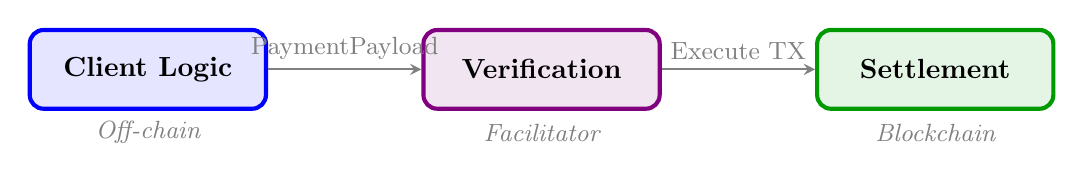
\begin{tikzpicture}[
    box/.style={
        rectangle,
        rounded corners=5pt,
        minimum width=3cm,
        minimum height=1cm,
        draw=#1,
        line width=1.5pt,
        fill=#1!10,
        font=\bfseries
    },
    arrow/.style={->, >=stealth, thick, gray}
]

\node[box=blue] (client) at (0,0) {Client Logic};
\node[box=violet] (verify) at (5,0) {Verification};
\node[box=green!60!black] (settle) at (10,0) {Settlement};

\draw[arrow] (client) -- node[above, font=\small] {PaymentPayload} (verify);
\draw[arrow] (verify) -- node[above, font=\small] {Execute TX} (settle);

\node[font=\small\itshape, gray] at (0,-0.8) {Off-chain};
\node[font=\small\itshape, gray] at (5,-0.8) {Facilitator};
\node[font=\small\itshape, gray] at (10,-0.8) {Blockchain};

\end{tikzpicture}
\caption{Payment scheme component flow}
\label{fig:scheme-flow}
\end{figure}

\section{Exact Scheme Overview}
\label{sec:exact-overview}

The \code{exact} scheme enables payments of a precise amount from payer to recipient.

\begin{definition}[Exact Scheme]
A payment scheme where the authorized transfer amount exactly equals the required payment amount, with no partial payments, refunds, or variability.
\end{definition}

\subsection{Properties}

\begin{table}[h]
\centering
\caption{Exact Scheme Properties}
\label{tab:exact-properties}
\begin{tabular}{lp{8cm}}
\toprule
\textbf{Property} & \textbf{Description} \\
\midrule
Deterministic & Payment amount known at request time \\
Atomic & Payment succeeds or fails completely \\
Non-custodial & Funds flow directly to recipient \\
Gasless & User pays no transaction fees (Facilitator sponsors) \\
Single-use & Each authorization can only be used once \\
Time-bounded & Authorizations expire after \code{validBefore} timestamp \\
\bottomrule
\end{tabular}
\end{table}

\subsection{Scheme Identifier}

The exact scheme is identified by \code{"scheme": "exact"} in payment requirements and payloads.

\section{EVM Implementation}
\label{sec:evm-implementation}

On EVM-compatible chains, the exact scheme uses EIP-3009 (Transfer with Authorization) for gasless, signature-based transfers.

\subsection{EIP-3009: Transfer with Authorization}

EIP-3009 defines a standard interface for token transfers authorized by cryptographic signatures rather than on-chain approval transactions:

\begin{lstlisting}[language=solidity,caption={EIP-3009 interface}]
interface IEIP3009 {
    function transferWithAuthorization(
        address from,
        address to,
        uint256 value,
        uint256 validAfter,
        uint256 validBefore,
        bytes32 nonce,
        uint8 v,
        bytes32 r,
        bytes32 s
    ) external;

    function authorizationState(
        address authorizer,
        bytes32 nonce
    ) external view returns (bool);
}
\end{lstlisting}

\subsection{Authorization Parameters}

\begin{table}[h]
\centering
\caption{EIP-3009 Authorization Parameters}
\label{tab:eip3009-params}
\begin{tabular}{llp{6cm}}
\toprule
\textbf{Parameter} & \textbf{Type} & \textbf{Description} \\
\midrule
\code{from} & address & Payer's wallet address \\
\code{to} & address & Recipient's wallet address (must match \code{payTo}) \\
\code{value} & uint256 & Transfer amount in atomic units \\
\code{validAfter} & uint256 & Unix timestamp when authorization becomes valid \\
\code{validBefore} & uint256 & Unix timestamp when authorization expires \\
\code{nonce} & bytes32 & Random 32-byte value for replay protection \\
\code{v, r, s} & uint8, bytes32, bytes32 & ECDSA signature components \\
\bottomrule
\end{tabular}
\end{table}

\subsection{EIP-712 Typed Data Signing}

The authorization uses EIP-712 structured signing for security and user experience:

\begin{lstlisting}[language=typescript,caption={EIP-712 domain and types}]
const domain = {
  name: tokenName,        // e.g., "USD Coin"
  version: tokenVersion,  // e.g., "2"
  chainId: chainId,       // e.g., 8453 for Base
  verifyingContract: tokenAddress
};

const types = {
  TransferWithAuthorization: [
    { name: "from", type: "address" },
    { name: "to", type: "address" },
    { name: "value", type: "uint256" },
    { name: "validAfter", type: "uint256" },
    { name: "validBefore", type: "uint256" },
    { name: "nonce", type: "bytes32" }
  ]
};
\end{lstlisting}

\subsection{Payload Structure}

The \code{payload} field for EVM exact scheme:

\begin{lstlisting}[language=json,caption={EVM exact scheme payload}]
{
  "signature": "0x2d6a7588...af148b571c",
  "authorization": {
    "from": "0x857b...36b66",
    "to": "0x2096...287C",
    "value": "10000",
    "validAfter": "1740672089",
    "validBefore": "1740672154",
    "nonce": "0xf374...3480"
  }
}
\end{lstlisting}

\subsection{Verification Algorithm}

\begin{algorithm}[H]
\caption{EVM Exact Scheme Verification}
\label{alg:evm-verification}
\SetKwInOut{Input}{Input}
\SetKwInOut{Output}{Output}
\Input{PaymentPayload $P$, PaymentRequirements $R$}
\Output{VerifyResponse}

\BlankLine
\tcp{Step 1: Signature Recovery}
$hash \gets \text{EIP712Hash}(P.authorization)$\;
$signer \gets \text{ecrecover}(hash, P.signature)$\;
\If{$signer \neq P.authorization.from$}{
    \Return{\{isValid: false, invalidReason: ``invalid\_signature''\}}\;
}

\BlankLine
\tcp{Step 2: Balance Verification}
$balance \gets \text{balanceOf}(R.asset, P.authorization.from)$\;
\If{$balance < R.amount$}{
    \Return{\{isValid: false, invalidReason: ``insufficient\_funds''\}}\;
}

\BlankLine
\tcp{Step 3: Amount Validation}
\If{$P.authorization.value < R.amount$}{
    \Return{\{isValid: false, invalidReason: ``invalid\_amount''\}}\;
}

\BlankLine
\tcp{Step 4: Recipient Validation}
\If{$P.authorization.to \neq R.payTo$}{
    \Return{\{isValid: false, invalidReason: ``invalid\_recipient''\}}\;
}

\BlankLine
\tcp{Step 5: Time Window Validation}
$now \gets \text{currentTimestamp}()$\;
\If{$now < P.authorization.validAfter$}{
    \Return{\{isValid: false, invalidReason: ``authorization\_not\_yet\_valid''\}}\;
}
\If{$now > P.authorization.validBefore$}{
    \Return{\{isValid: false, invalidReason: ``expired\_authorization''\}}\;
}

\BlankLine
\tcp{Step 6: Nonce Validation}
$used \gets \text{authorizationState}(P.authorization.from, P.authorization.nonce)$\;
\If{$used$}{
    \Return{\{isValid: false, invalidReason: ``nonce\_already\_used''\}}\;
}

\BlankLine
\tcp{Step 7: Transaction Simulation}
$result \gets \text{eth\_call}(\text{transferWithAuthorization}, P)$\;
\If{$result.reverted$}{
    \Return{\{isValid: false, invalidReason: ``simulation\_failed''\}}\;
}

\Return{\{isValid: true, payer: $P.authorization.from$\}}\;
\end{algorithm}

\subsection{Settlement Process}

Upon successful verification, the Facilitator executes settlement:

\begin{enumerate}
    \item Construct the \code{transferWithAuthorization} transaction
    \item Sign with the Facilitator's hot wallet (for gas payment)
    \item Broadcast to the network
    \item Wait for confirmation (typically 1-2 blocks on L2)
    \item Return transaction hash in \code{SettlementResponse}
\end{enumerate}

\section{Solana (SVM) Implementation}
\label{sec:solana-implementation}

On Solana, the exact scheme uses SPL Token \code{TransferChecked} instructions with Facilitator-sponsored fee payment.

\subsection{Transaction Structure}

Solana payments require a specific instruction layout:

\begin{table}[h]
\centering
\caption{Required Solana Transaction Instructions}
\label{tab:solana-instructions}
\begin{tabular}{clp{6cm}}
\toprule
\textbf{Index} & \textbf{Program} & \textbf{Instruction} \\
\midrule
0 & ComputeBudget & SetComputeUnitLimit \\
1 & ComputeBudget & SetComputeUnitPrice \\
2 & Token/Token2022 & TransferChecked \\
\bottomrule
\end{tabular}
\end{table}

\subsection{Payload Structure}

\begin{lstlisting}[language=json,caption={Solana exact scheme payload}]
{
  "transaction": "AQAAAAAAAAAAAAAA...base64-encoded..."
}
\end{lstlisting}

The \code{transaction} field contains a Base64-encoded, serialized, \textbf{partially-signed} versioned Solana transaction. The client signs as the token authority; the Facilitator adds its signature as the fee payer.

\subsection{PaymentRequirements Extra Fields}

\begin{lstlisting}[language=json,caption={Solana-specific extra fields}]
{
  "extra": {
    "feePayer": "EwWqGE4ZFKLofuestmU4LDdK7XM1N4ALgdZccwYugwGd"
  }
}
\end{lstlisting}

\subsection{Facilitator Security Rules}

\begin{securitybox}[Critical Security Checks for Solana]
The Facilitator \textbf{MUST} enforce all of the following:

\begin{enumerate}
    \item \textbf{Instruction Layout}: Exactly 3 instructions in the specified order
    \item \textbf{Fee Payer Safety}: Fee payer address must NOT appear in any instruction accounts
    \item \textbf{Authority Safety}: Fee payer must NOT be the transfer authority or source
    \item \textbf{Compute Price Bound}: Compute unit price $\leq$ 5 lamports per CU
    \item \textbf{Destination Validation}: Destination must equal the ATA PDA for (payTo, asset)
    \item \textbf{Amount Exactness}: Transfer amount must exactly equal requirements amount
\end{enumerate}
\end{securitybox}

\section{TON Implementation}
\label{sec:ton-implementation}

On TON, payments use Jetton (TON's fungible token standard) transfers.

\subsection{Jetton Transfer Message}

TON Jettons use an internal message-based transfer mechanism:

\begin{lstlisting}[caption={TON Jetton transfer cell structure}]
transfer#0f8a7ea5
  query_id:uint64
  amount:(VarUInteger 16)
  destination:MsgAddress
  response_destination:MsgAddress
  custom_payload:(Maybe ^Cell)
  forward_ton_amount:(VarUInteger 16)
  forward_payload:(Either Cell ^Cell)
= InternalMsgBody;
\end{lstlisting}

\subsection{Payload Structure}

\begin{lstlisting}[language=json,caption={TON exact scheme payload}]
{
  "boc": "te6ccgEBAgEAhgAB...base64-encoded-BOC..."
}
\end{lstlisting}

\subsection{Verification Requirements}

\begin{itemize}
    \item Validate Ed25519 signature
    \item Verify sender wallet address matches authorization
    \item Check Jetton master contract address
    \item Validate workchain ID (0 for basechain)
    \item Verify sufficient balance
\end{itemize}

\section{TRON Implementation}
\label{sec:tron-implementation}

On TRON, payments use TRC-20 token transfers.

\subsection{Transaction Structure}

TRON uses Protobuf-encoded transactions with ECDSA secp256k1 signatures.

\subsection{Payload Structure}

\begin{lstlisting}[language=json,caption={TRON exact scheme payload}]
{
  "transaction": "0a02...hex-encoded-protobuf...",
  "signature": "0x..."
}
\end{lstlisting}

\subsection{Special Considerations}

\begin{itemize}
    \item \textbf{Energy/Bandwidth}: TRON uses energy and bandwidth instead of gas
    \item \textbf{Address Format}: Base58Check encoding (starts with 'T')
    \item \textbf{Contract Address}: Official USDT: \code{TR7NHqjeKQxGTCi8q8ZY4pL8otSzgjLj6t}
\end{itemize}

\section{Scheme Comparison}
\label{sec:scheme-comparison}

\begin{table}[h]
\centering
\caption{Exact Scheme Implementation Comparison}
\label{tab:scheme-comparison}
\begin{tabular}{lllll}
\toprule
\textbf{Aspect} & \textbf{EVM} & \textbf{Solana} & \textbf{TON} & \textbf{TRON} \\
\midrule
Signature & ECDSA & Ed25519 & Ed25519 & ECDSA \\
Standard & EIP-3009 & SPL Token & Jetton & TRC-20 \\
Nonce & 32 bytes & N/A (tx sig) & query\_id & N/A \\
Gasless & Native & Fee sponsor & Fee sponsor & Energy \\
Finality & $\sim$2s (L2) & $\sim$0.4s & $\sim$5s & $\sim$3s \\
\bottomrule
\end{tabular}
\end{table}

\section{Future Schemes}
\label{sec:future-schemes}

\subsection{Up-To Scheme}

The planned ``up-to'' scheme will support metered payments:

\begin{itemize}
    \item \textbf{Mechanism}: EIP-2612 (Permit) for EVM
    \item \textbf{Use Case}: Pay for actual usage up to a maximum
    \item \textbf{Settlement}: Partial settlement of authorized amount
\end{itemize}

\begin{lstlisting}[language=json,caption={Up-to scheme requirements (proposed)}]
{
  "scheme": "up-to",
  "network": "eip155:8453",
  "maxAmount": "1000000",
  "asset": "0x...",
  "payTo": "0x..."
}
\end{lstlisting}

\subsection{Permit2 Integration}

Uniswap's Permit2 offers improved efficiency:

\begin{itemize}
    \item Single approval for multiple protocols
    \item Batch transfers
    \item Expiring approvals for better security
\end{itemize}
